% Beyond the Road Toll -- COS30045 project pitch. Build: latexmk -pdf beyond_the_road_toll.tex
\documentclass[aspectratio=169,14pt]{beamer}
\usepackage[T1]{fontenc}
\usepackage{sourcesans}
\usepackage{sourceserif}
\usepackage{microtype}
\usepackage{array}
\usepackage{tikz}
\usetikzlibrary{positioning,arrows.meta,calc,shapes.misc}

% ---------- palette (website/css/style.css) ----------
\definecolor{paper}{HTML}{FAF8F3}
\definecolor{ink}{HTML}{1C2230}
\definecolor{inktwo}{HTML}{434A5A}
\definecolor{muted}{HTML}{646B78}
\definecolor{rule}{HTML}{D9D4C8}
\definecolor{band}{HTML}{ECE8DC}
\definecolor{accent}{HTML}{B8470F}
\definecolor{accentsoft}{HTML}{F4D8C5}
\definecolor{accentink}{HTML}{8F3406}
\definecolor{blue}{HTML}{1F5F99}
\definecolor{bluesoft}{HTML}{CFE0EF}

% ---------- minimal theme ----------
\setbeamercolor{background canvas}{bg=paper}
\setbeamercolor{normal text}{fg=ink}
\setbeamercolor{structure}{fg=accent}
\setbeamertemplate{navigation symbols}{}
\setbeamertemplate{itemize item}{\color{accent}\textbullet}
\setbeamersize{text margin left=11mm,text margin right=11mm}
\setbeamerfont{normal text}{family=\sffamily}
\newcommand{\serif}{\rmfamily}
\setbeamertemplate{frametitle}{%
  \vskip 4.5mm
  \begin{minipage}[t][8mm][t]{\textwidth}\raggedright
    {\serif\bfseries\fontsize{19}{21}\selectfont\color{ink}\insertframetitle\par}
  \end{minipage}\vskip 0mm}
\setbeamertemplate{footline}{%
  \hbox to\paperwidth{\hspace{11mm}{\fontsize{8}{9}\sffamily\color{muted}Beyond the Road Toll \;\textperiodcentered\; COS30045}\hfill
  {\fontsize{9}{10}\sffamily\bfseries\color{accentink}\insertframenumber}\hspace{11mm}}\vskip 3.2mm}
\setbeamertemplate{headline}{\begin{tikzpicture}[remember picture,overlay]
  \fill[accent] (current page.north west)++(11mm,-3.5mm) rectangle ++(9mm,-0.9mm);\end{tikzpicture}}

% source line, bottom of slide, above footer
\newcommand{\source}[1]{\begin{tikzpicture}[remember picture,overlay]
  \node[anchor=south west,text width=138mm,inner sep=0,align=left] at ($(current page.south west)+(11mm,8.3mm)$)
  {\raggedright\fontsize{7.5}{8.5}\sffamily\color{muted}Source: #1\par};\end{tikzpicture}}
\newcommand{\kicker}[1]{{\fontsize{9}{10}\sffamily\bfseries\color{accentink}\MakeUppercase{#1}}}
\newcommand{\bignum}[2]{{\serif\bfseries\fontsize{#1}{#1}\selectfont #2}}
\newcommand{\rtag}[2]{\colorbox{#1}{\strut\,\fontsize{11}{12}\sffamily\bfseries #2\,}}

\title{Beyond the Road Toll}
\hypersetup{pdftitle={Beyond the Road Toll},pdfauthor={COS30045 Team}}
\begin{document}

% 1 ---------------------------------------------------------------- title
\begin{frame}[plain]
\begin{tikzpicture}[remember picture,overlay]
  \fill[accent] (current page.north west)++(11mm,-14mm) rectangle ++(14mm,-1.4mm);
  \node[anchor=north west,text width=135mm,inner sep=0] at ($(current page.north west)+(11mm,-20mm)$) {%
    \kicker{A data story \;\textperiodcentered\; project pitch}\\[3mm]
    {\serif\bfseries\fontsize{40}{42}\selectfont Beyond the\\[-1mm] Road Toll}\\[4mm]
    {\fontsize{16}{20}\sffamily\color{inktwo}Hospitalised injuries from road crashes\\ in Australia, 2011--2021}};
  \node[anchor=south west,inner sep=0] at ($(current page.south west)+(11mm,10mm)$)
    {\fontsize{12}{14}\sffamily\color{muted}COS30045 Data Visualisation \;\textperiodcentered\; Team [Team names]};
\end{tikzpicture}
\end{frame}

% 2 ------------------------------------------------------------------ hook
\begin{frame}{For every death, 35 hospitalised (27 in 2011)}
\vspace{1mm}
\begin{columns}[T,onlytextwidth]
 \column{0.56\textwidth}
  \bignum{34}{\color{accent}39,505}\\[-1mm]
  {\fontsize{13}{15}\sffamily hospitalised in 2021 (about 108 a day)}
 \column{0.4\textwidth}
  \bignum{34}{\color{ink}1,130}\\[-1mm]
  {\fontsize{13}{15}\sffamily road deaths in 2021}
\end{columns}
\vspace{1mm}
\centering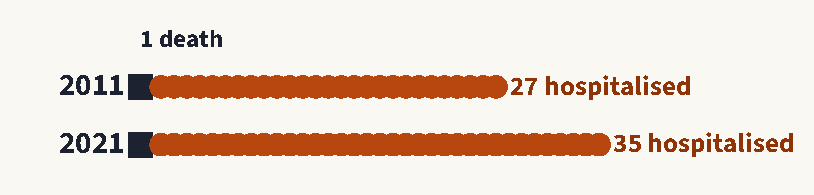
\includegraphics[width=\textwidth]{figures/hook_units.pdf}
\source{BITRE Hospitalised injury data (Sep 2023); BITRE Australian Road Deaths Database. Hospitalised per death.}
\end{frame}

% 3 --------------------------------------------------------------- audience
\begin{frame}{Who we are telling it to}
\begin{columns}[T,onlytextwidth]
 \column{0.52\textwidth}
  \kicker{Primary reader}\\[1mm]
  {\serif\bfseries\fontsize{26}{28}\selectfont Sam, 52}\\[0mm]
  {\sffamily Outer-suburban Brisbane. Drives to work, took up weekend cycling in 2020, parents in their late 70s.}
 \column{0.46\textwidth}
  \kicker{Sam's two questions}\\[1.5mm]
  {\serif\itshape\fontsize{17}{20}\selectfont ``Is it getting safer out there?''}\\[2mm]
  {\serif\itshape\fontsize{17}{20}\selectfont ``Is that true for people like me, and my parents?''}
\end{columns}
\vfill
\begin{tikzpicture}\draw[rule,line width=0.6pt] (0,0)--(\textwidth,0);\end{tikzpicture}\\[1.5mm]
{\sffamily\fontsize{14}{17}\selectfont\color{inktwo}\textbf{Also reading:} councillors, road-safety advocates and health planners.}
\vspace{9mm}
\end{frame}

% 4 -------------------------------------------------------------------- RQs
\begin{frame}{Five questions, two already answered}
\renewcommand{\arraystretch}{1.25}
\fontsize{13}{15}\selectfont\sffamily
\begin{tabular}{@{}l@{\hspace{2mm}}>{\raggedright\arraybackslash}p{80mm}@{\hspace{2mm}}l@{}}
 \textbf{RQ1} & Is progress real once we count the injured, not just the dead? & \rtag{accent}{\color{white}Phase 1: built}\\
 \textbf{RQ2} & Who is the new face of road injury? & \rtag{accent}{\color{white}Phase 1: built}\\
 \textbf{RQ3} & Which crashes do the most damage: volume vs severity? & \rtag{accentsoft}{\color{accentink}Partly in Phase 1}\\
 \textbf{RQ4} & What did the 2020 lockdowns reveal? (natural experiment) & \rtag{band}{\color{inktwo}Phase 2}\\
 \textbf{RQ5} & Equity: First Nations people and remoteness. & \rtag{band}{\color{inktwo}Phase 2}\\
\end{tabular}
\end{frame}

% 5 ----------------------------------------------------------- divider 1
\begin{frame}[plain]
\begin{tikzpicture}[remember picture,overlay]
 \fill[ink] (current page.north west) rectangle (current page.south east);
 \node[anchor=north west,text width=135mm,inner sep=0] at ($(current page.north west)+(11mm,-18mm)$) {%
  {\fontsize{10}{12}\sffamily\bfseries\color{accentsoft}\MakeUppercase{Idea 1}}\\[3mm]
  {\serif\bfseries\fontsize{30}{34}\selectfont\color{paper}The road toll is falling.\\ \color{accentsoft}The injury toll isn't.}};
\end{tikzpicture}
\end{frame}

% 6 ------------------------------------------------------------ index chart
\begin{frame}{Hospitalisations rose; deaths fell}
\centering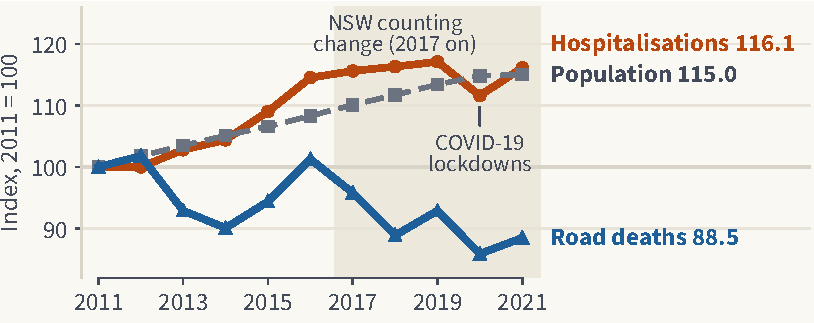
\includegraphics[width=\textwidth]{figures/index_counts.pdf}
\source{BITRE Hospitalised injury data (Sep 2023); ABS ERP; BITRE ARDD. Indexed to 2011 = 100.}
\end{frame}

% 7 ---------------------------------------------------------- per person
\begin{frame}{Per person: deaths down, injuries flat}
\begin{columns}[T,onlytextwidth]
 \column{0.485\textwidth}
  \kicker{Hospitalised per 100,000}\\[0.5mm]
  \bignum{22}{\color{accent}152.3 \textrightarrow{} 153.8}\\[-0.5mm]
  {\fontsize{13}{14}\sffamily\bfseries\color{accentink}Flat since 2011}\\[0mm]
  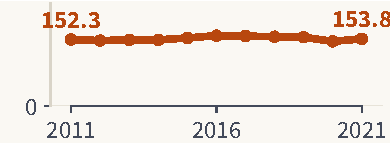
\includegraphics[width=\textwidth]{figures/rate_hosp.pdf}
 \column{0.485\textwidth}
  \kicker{Road deaths per 100,000}\\[0.5mm]
  \bignum{22}{\color{blue}5.72 \textrightarrow{} 4.40}\\[-0.5mm]
  {\fontsize{13}{14}\sffamily\bfseries\color{blue}Down 23\%}\\[0mm]
  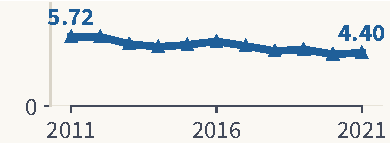
\includegraphics[width=\textwidth]{figures/rate_deaths.pdf}
\end{columns}
\vspace{0mm}
{\serif\itshape\fontsize{13}{15}\selectfont Fewer people are dying; the same share of us are still being badly hurt.}
\source{BITRE Hospitalised injury data (Sep 2023); ABS ERP; BITRE ARDD. Rates per 100,000.}
\end{frame}

% 8 ----------------------------------------------------------- divider 2
\begin{frame}[plain]
\begin{tikzpicture}[remember picture,overlay]
 \fill[ink] (current page.north west) rectangle (current page.south east);
 \node[anchor=north west,text width=135mm,inner sep=0] at ($(current page.north west)+(11mm,-16mm)$) {%
  {\fontsize{10}{12}\sffamily\bfseries\color{accentsoft}\MakeUppercase{Idea 2}}\\[3mm]
  {\serif\bfseries\fontsize{27}{31}\selectfont\color{paper}Older riders, longer stays:\\ \color{accentsoft}cycling injuries have more than doubled among over-65s.}};
\end{tikzpicture}
\end{frame}

% 9 --------------------------------------------------------------- heatmap
\begin{frame}{Cyclists over 65 are the hot spot}
\centering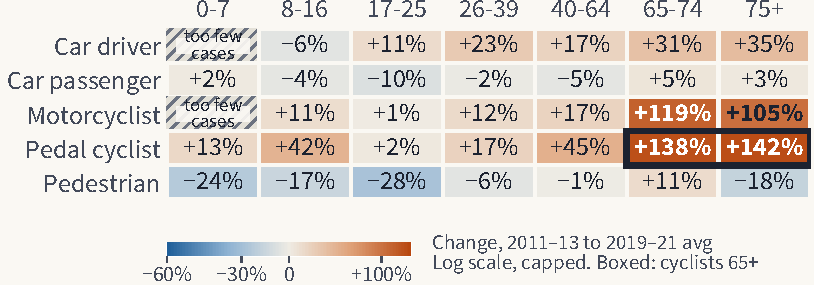
\includegraphics[width=\textwidth]{figures/heatmap.pdf}\\
{\raggedright\fontsize{11}{12}\sffamily\color{inktwo}On the website, a ``Find yourself'' explorer lets Sam pick a road user and age group.\par}
\source{BITRE Hospitalised injury data (Sep 2023), traffic only. Hatched: too few cases.}
\end{frame}

% 10 -------------------------------------------------- counts vs per person
\begin{frame}{Ageing explains part of it, not all}
\centering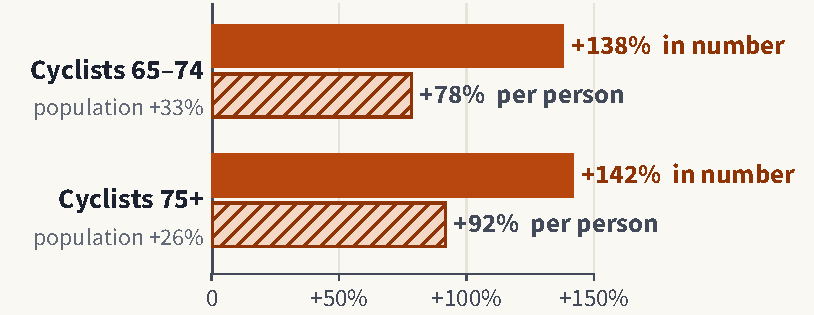
\includegraphics[width=\textwidth]{figures/counts_vs_rate.pdf}
\source{BITRE Hospitalised injury data (Sep 2023); ABS ERP. 2011--13 average to 2019--21 average. Per person = (1 + change in count) / (1 + change in population) \textminus{} 1.}
\end{frame}

% 11 -------------------------------------------------------------- severity
\begin{frame}{Over-75s stay 2.6\texttimes{} longer and die 8\texttimes{} as often}
\centering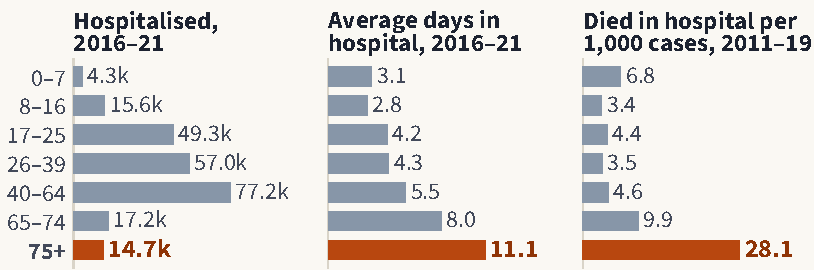
\includegraphics[width=\textwidth]{figures/severity.pdf}\\
{\raggedright\fontsize{11.5}{13}\sffamily\color{inktwo}\textbf{75+:} 11.1 days vs 4.3 (ages 26--39); 28.1 vs 3.5 deaths per 1,000.\par}
\source{BITRE Hospitalised injury data (Sep 2023). Stays within 2016--21; deaths 2011--19 (2020--21 incomplete).}
\end{frame}

% 12 -------------------------------------------------------------- pipeline
\begin{frame}{From raw spreadsheets to a trustworthy chart}
\tikzset{
  box/.style={rounded corners=2pt,draw=ink,line width=0.7pt,fill=white,align=center,font=\fontsize{11.5}{12.5}\sffamily,inner sep=3pt,minimum height=10mm,text width=28mm},
  hl/.style={box,fill=accentsoft,draw=accent},
  arr/.style={-{Stealth[length=2.2mm]},line width=0.9pt,color=inktwo}}
\centering
\begin{tikzpicture}
 \node[box] (raw) at (0,0) {BITRE raw\\Excel tabs};
 \node[box] (clean) at (3.65,0) {\textbf{Cleaning}\\[-0.5mm]{\small Python + KNIME}};
 \node[hl] (val) at (7.3,0) {\textbf{Validation}\\[-0.5mm]{\small totals match T1--T4}};
 \node[box] (csv) at (10.95,0) {Tidy CSVs};
 \node[box] (ard) at (3.65,-1.5) {BITRE road deaths};
 \node[box] (abs) at (7.3,-1.5) {ABS population};
 \node[hl] (web) at (10.95,-1.5) {D3 website};
 \draw[arr] (raw)--(clean); \draw[arr] (clean)--(val); \draw[arr] (val)--(csv);
 \draw[arr] (ard)--(abs); \draw[arr] (abs)--(web); \draw[arr] (csv)--(web);
\end{tikzpicture}\\[2mm]
{\raggedright\fontsize{12}{14}\sffamily\color{inktwo}\textbf{Eleven cleaning rules,} including: traffic crashes only; the \textit{Hospitalisations} column; series-break flags; bed days 2016--21; deaths 2011--19; small-count flags.\par}
\source{BITRE Hospitalised injury data (Sep 2023); ABS ERP; BITRE ARDD. Code: \texttt{processing/clean\_data.py}.}
\end{frame}

% 13 --------------------------------------------------------------- caveats
\begin{frame}{We say what the data cannot say}
\tikzset{card/.style={rounded corners=2pt,fill=white,draw=rule,line width=0.8pt,text width=43mm,minimum height=19mm,inner sep=5pt,align=left,font=\fontsize{12}{13.5}\sffamily,anchor=north west}}
\centering
\begin{tikzpicture}
 \node[card] at (0,0) {\textbf{\color{accentink}Counts are not rates}\\ Hence the per-person toggles.};
 \node[card] at (4.8,0) {\textbf{\color{accentink}Counting changes}\\ Victoria 2012, NSW 2017.};
 \node[card] at (9.6,0) {\textbf{\color{accentink}Bed-day method}\\ Changed July 2015, so compare 2016--21.};
 \node[card] at (0,-2.2) {\textbf{\color{accentink}Deaths in care}\\ Incomplete for 2020--21.};
 \node[card] at (4.8,-2.2) {\textbf{\color{accentink}Home, not crash site}\\ Location is where the patient lives.};
 \node[card] at (9.6,-2.2) {\textbf{\color{accentink}No exposure data}\\ We cannot see how much people ride.};
\end{tikzpicture}
\source{BITRE Hospitalised injury data dictionary (Sep 2023); HANDOFF data caveats.}
\end{frame}

% 14 --------------------------------------------------------------- website
\begin{frame}{What the reader gets}
\begin{columns}[T,onlytextwidth]
 \column{0.43\textwidth}
  \fontsize{13}{16}\selectfont\sffamily
  \textbf{Five D3 charts} in two chapters\\[1.5mm]
  \textbf{``Find yourself''} explorer\\[1.5mm]
  \textbf{Counts or per-person} toggles\\[1.5mm]
  \textbf{Mobile first, accessible:} data tables, colour-blind palette\\[1.5mm]
  \textbf{Methods section} on every caveat
 \column{0.55\textwidth}
  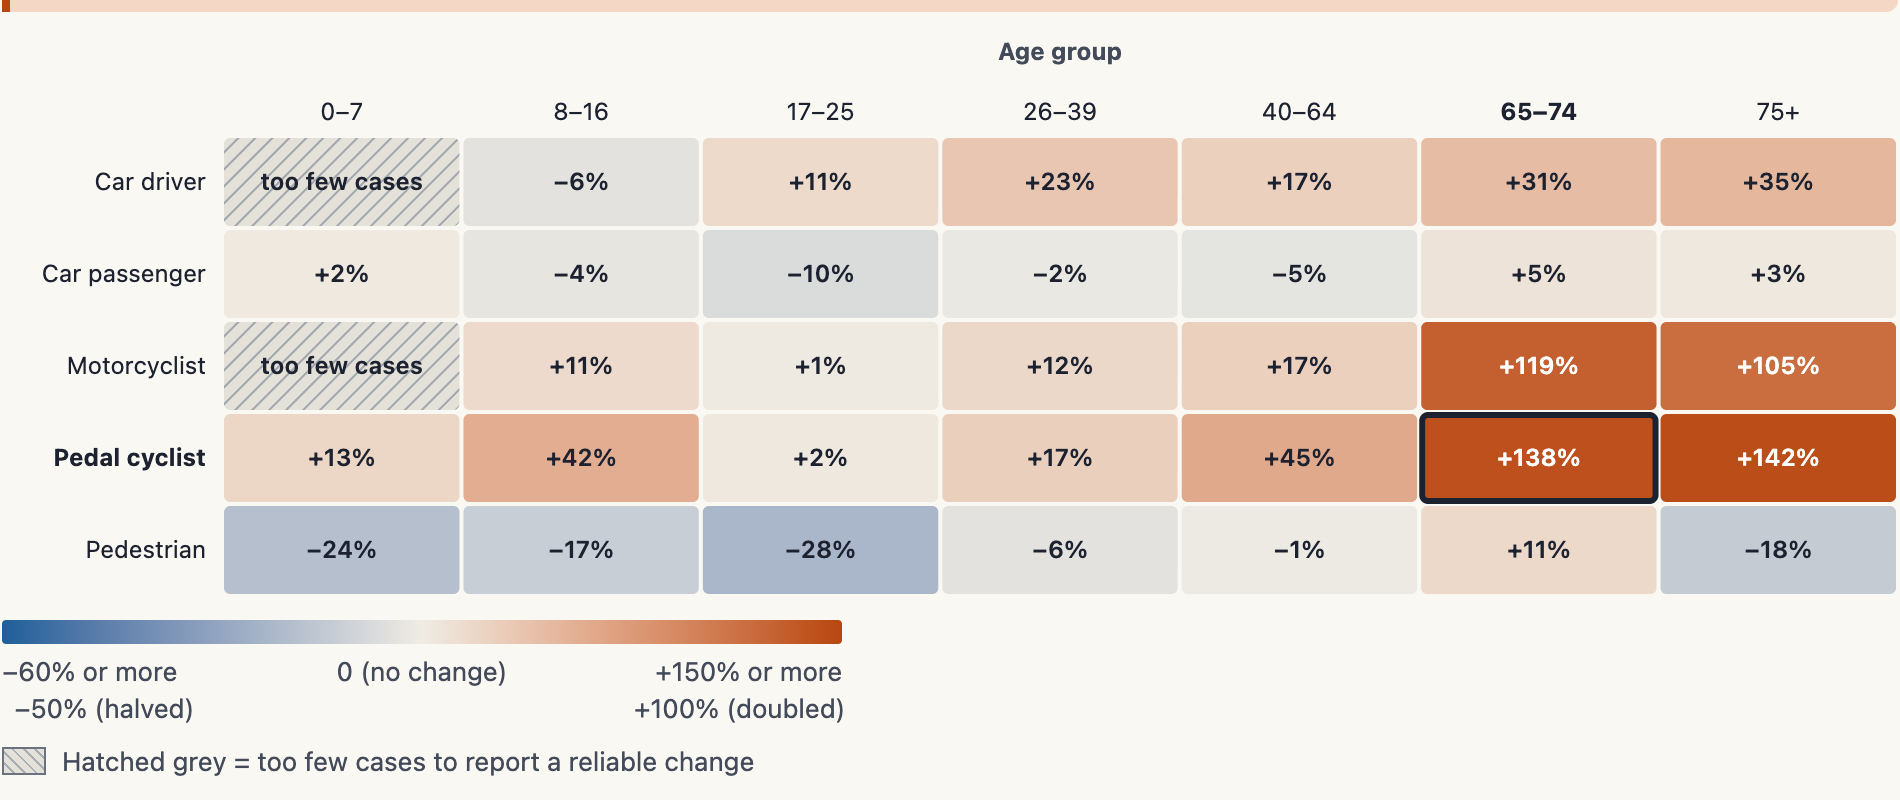
\includegraphics[width=\textwidth]{figures/website_heatmap.png}\\[1mm]
  {\fontsize{10}{11}\sffamily\color{muted}The ``Find yourself'' heatmap on the website}
\end{columns}
\end{frame}

% 15 ------------------------------------------------------------ next steps
\begin{frame}{Next steps}
\begin{columns}[T,onlytextwidth]
 \column{0.31\textwidth}
  \kicker{1 \;\textperiodcentered\; Test}\\[1mm]
  {\serif\bfseries\fontsize{16}{18}\selectfont Usability testing}\\[1.5mm]
  {\fontsize{13}{15.5}\sffamily Think-aloud with 5--6 Sam-like participants. Task success, time on task, SUS.}
 \column{0.31\textwidth}
  \kicker{2 \;\textperiodcentered\; Extend}\\[1mm]
  {\serif\bfseries\fontsize{16}{18}\selectfont Phase 2 chapters}\\[1.5mm]
  {\fontsize{13}{15.5}\sffamily Pedestrians, the 2020 lockdowns, First Nations and remoteness.}
 \column{0.31\textwidth}
  \kicker{3 \;\textperiodcentered\; Ship}\\[1mm]
  {\serif\bfseries\fontsize{16}{18}\selectfont Mercury deployment}\\[1.5mm]
  {\fontsize{13}{15.5}\sffamily Host the finished story on the Swinburne Mercury server.}
\end{columns}
\end{frame}

% 16 --------------------------------------------------------------- sources
\begin{frame}{Sources}
\fontsize{13}{16}\selectfont\sffamily
\textbf{BITRE.} Hospitalised injury data, September 2023.\\[2.5mm]
\textbf{ABS.} Estimated Resident Population (dataflow ERP\_Q), CC BY 4.0.\\[2.5mm]
\textbf{BITRE.} Australian Road Deaths Database, via data.gov.au (October 2023 file), CC BY 3.0 AU.
\end{frame}

\end{document}
